\section{Entropia}

\epigraph{\justifying Para encontrar um nome para esta função, Clausius disse
\begin{displayquote}
    Eu prefiro me basear em línguas antigas para o nome de grandezas científicas
    importantes, de forma que elas signifiquem a mesma coisa em todas as línguas
    vivas. Assim, eu proponho chamar $S$ de \emph{entropia} de um corpo, da
    palavra grega "transformação". Eu intencionalmente cunhei a palavra \emph{
    entropia} de forma a ser similar a energia, dado que essas duas grandezas
    são tão análogas em seu significado físico que uma analogia de denominação
    me parece muito útil.
\end{displayquote}
Com isso, ao contrário do que aconteceria se extraisse um nome do corpo da
linguagem contemporânea (como calor perdido), ele conseguiu cunhar um termo que
tem o mesmo significado para todo mundo: nenhum.}{\emph{Leon N. Cooper}, An
Introduction to the Meaning and Structure of Physics (1968)}

\subsection{Ciclos termodinâmicos}

Dado um sistema físico, podemos realizar uma sequência de processos
termodinâmicos encadeados que eventualmente resultam no sistema retornando ao
seu estado inicial, isto é, de forma que todas as variáveis de estado do sistema
sejam iguais antes e depois da sequência de processos. Tal sequência de
processos recebe o nome de \emph{ciclo termodinâmico}. Denotando cada um dos
processos por um índice $i$, podemos também denotar o calor $Q_i$ e trabalho
$W_i$ recebidos pelo sistema, que totalizam
$$Q_\text{tot}=\sum_iQ_i,\quad W_\text{tot}=\sum_iW_i,$$
e da primeira lei da termodinâmica devemos concluir que
$$\Delta U=Q_\text{tot}+W_\text{tot}=0.$$

De maneira geral vamos sempre supor que a divisão em processos $i$ é refinada o
suficiente de forma que o sinal de $Q_i$ caracteriza o processo no seguinte
sentido. Se $Q_i>0$ o processo apenas absorve calor, e se $Q_i<0$ o processo
apenas libera calor. Assim, podemos separar o calor em entradas e saídas como
$$Q_\text{in}=\sum_{Q_i>0}Q_i,\quad Q_\text{out}=-\sum_{Q_i<0}Q_i$$
e escrever $Q_\text{tot}=-W_\text{tot}=Q_\text{in}-Q_\text{out}$. Por sua vez, o
sinal de $W_\text{tot}$ será utilizado para dividir ciclos termodinâmicos em
dois grandes grupos. Quando $W_\text{tot}<0$, estamos utilizando energia na
forma de calor para realizar trabalho num meio externo, sendo um \emph{ciclo de 
potência} ou \emph{máquina térmica}. Quando $W_\text{tot}>0$ estamos
utilizando energia na forma de trabalho para trasferir calor num meio externo,
sendo um \emph{ciclo de refrigeração} ou \emph{bomba de calor}. Ambas as classes
de ciclos possuem noções de eficiência correspondentes. Para máquinas térmicas 
definimos o \emph{rendimento}
$$\eta=-\frac{W_\text{tot}}{Q_\text{in}},$$
enquanto para bombas de calor definimos o \emph{coeficiente de performance}, e a
noção vai depender se o ciclo é usado como refrigerador, onde o calor de
interesse é o absorvido
$$\mu_\text{cool}=\frac{Q_\text{in}}{W_\text{tot}},$$
ou como aquecedor, onde o calor de interesse é o liberado
$$\mu_\text{heat}=\frac{Q_\text{out}}{W_\text{tot}}=\mu_\text{cool}+1.$$

\subsection{A Segunda Lei}

Aqui começamos a lidar com a possibilidade de processos físicos que não podem
ser "desfeitos" de uma maneira trivial. Um mergulhador olímpico pode saltar e
cair na piscina, dissipando sua energia na água, mas não vemos a água se
organizando para empurrá-lo de volta para a prancha. Um balão de hélio ao
estourar espalha suas moléculas pela atmosfera, mas não vemos elas voltando para
a região original e expulsando o ar em volta de maneira espontânea. Uma cápsula
espacial caindo pela atmosfera é freada pela resistência do ar e entra em
chamas, mas não vemos o ar absorvendo essas chamas e catapultando a cápsula de
volta para a órbita. 

Todos os processos acima são chamados \emph{irreversíveis}, ou seja, apesar de
ser possível retornar o sistema de interesse para o estado em que estava antes
do processo, é necessária a intervenção de algum outro sistema, normalmente na
forma de trabalho. O mergulhador precisa subir novamente as escadas da prancha.
Precisamos bombear uma quantidade de hélio para dentro de um balão. Precisamos
de um foguete para lançar a cápsula espacial. 

Enquanto a todos os processos macroscópicos na natureza são irreversíveis, a
estrutura matemática da termodinâmica se beneficia muito ao considerarmos
processos idealizados \emph{reversíveis}. São aqueles que, se levam o sistema de
um estado $i$ até um estado $f$ absorvendo calor $Q$ e recebendo trabalho $W$,
existe um processo que leva do estado $f$ até o estado $i$ liberando calor $Q$
(absorvendo $-Q$) e realizando trabalho $W$ (recebendo $-W$). Note que um ciclo
termodinâmico será reversível quando todos os processos envolvidos são
reversíveis também.

Se definirmos um \emph{reservatório térmico} como um sistema termodinâmico tão
grande, a ponto de que sua capacidade térmica seja efetivamente infinita nas
escalas de energia que estamos interessados, podemos introduzir a seguinte lei
física enunciada por Kelvin em 1851, e reformulada por Planck em 1903:
\begin{law}[Kelvin-Planck]
    Não existe uma máquina térmica que consegue operar trocando calor com um
    único reservatório térmico.
\end{law}
Ou seja, se um sistema realiza algum ciclo termodinâmico em contato com um
único reservatório, o sistema necessariamente deve absorver trabalho ao invés de
realizá-lo.

O que acontece então no caso de dois reservatórios? Vamos considerar um ciclo
que em cada passo pode trocar calor com um de dois reservatórios a temperaturas
$\theta_C$ e $\theta_H$, com os nomes escolhidos de forma que o calor total
recebido de $\theta_H$ pelo sistema é positivo. Então vale o seguinte

\begin{theorem}[Carnot]
    Existe uma função única $g$ da temperatura do reservatório de forma que o
    rendimento de um ciclo termodinâmico satisfaz
    $$\eta\leq1-\frac{g(\theta_C)}{g(\theta_H)}.$$
    Temos igualdade no caso em que o ciclo é reversível, recebendo o nome de
    cíclo de Carnot.
\end{theorem}
Note que a função $g$ é uma escala de temperatura, que recebe o nome especial de
\emph{temperatura termodinâmica} $T=g(\theta)$. É fácil ver que dois
reservatórios com diferentes sinais para a temperatura levam a uma violação da
Segunda Lei, e portanto vamos convencionar que todos eles possuem temperatura
positiva. Note que o teorema de Carnot também nos mostra que a troca de calor
entre dois sistemas a temperaturas termodinâmicas diferentes é sempre
irreversível, e também a uma formulação equivalente da Segunda Lei como

\setcounter{law}{1}
\begin{law}[Clausius]
    Não existe um processo termodinâmico cujo único resultado é a transferência
    de calor de um corpo frio para um corpo quente.
\end{law}

O resultado generaliza imediatamente para muitos reservatórios, e é também
devido ao
\begin{theorem}[Clausius]
    Se um ciclo termodinâmico possui passos $i$ onde recebe calor $Q_i$ de um
    reservatório à temperatura $T_i$ vale que
    $$\sum_i\frac{Q_i}{T_i}\leq0,$$
    com igualdade num ciclo reversível.
\end{theorem}

Prestemos muita atenção no caso de igualdade. Ele nos mostra que para qualquer
sequência de processos reversíveis, onde precisamos que a temperatura do sistema
seja igual à do reservatório de onde recebe calor, o somatório do teorema zera.
Podemos enfim concluir que deve existir uma variável de estado $S$, chamada
\emph{entropia}, definida para qualquer sistema termodinâmico de forma que, em
qualquer isoterma $T$ onde o sistema absorve calor $Q$,
$$\Delta S=\frac{Q}{T}.$$
No caso de processos contínuos gerais, que são sempre reversíveis, a expressão
acima vale em forma diferencial
$$dS=\frac{\delta Q}{T}.$$
Podemos também escrever o enunciado moderno da Segunda Lei, que também é o mais
conhecido no meio leigo apesar da elusividade da definição de entropia em si.
\setcounter{law}{1}
\begin{law}[Entropia]
    Para um sistema isolado, os únicos processos termodinâmicos possíveis são
    aqueles que acarretam um aumento da entropia total. Um processo é reversível
    se, e somente se não acarreta em variação da entropia total.
\end{law}

Munidos com a definição de entropia, podemos também obter uma representação
gráfica para um cíclo reversível de Carnot no diagrama $TS$, composto de duas
isotermas e duas adiabáticas:
\begin{figure}[H]
    \centering
    \begin{tikzpicture}
        \draw[->, thick]
            (0,0) -- (5,0) node[below] {$S$};
        \draw[->, thick]
            (0,0) -- (0,4) node[left] {$T$};
        \draw
            (1.5,0.2) -- (1.5,-0.2) node[below] {$S_\text{min}$};
        \draw
            (3.5,0.2) -- (3.5,-0.2) node[below] {$S_\text{max}$};
        \draw
            (0.2,1.2) -- (-0.2,1.2) node[left] {$T_C$};
        \draw
            (0.2,2.8) -- (-0.2,2.8) node[left] {$T_H$};
        \fill[lightgray]
            (1.5,1.2) -- (1.5,2.8) -- (3.5,2.8) -- (3.5,1.2) -- cycle;
        \draw[ultra thick,postaction={mid arrow}]
            (1.5,1.2) -- (1.5,2.8);
        \draw[ultra thick,postaction={mid arrow}]
            (1.5,2.8) -- (3.5,2.8);
        \draw[ultra thick,postaction={mid arrow}]
            (3.5,2.8) -- (3.5,1.2);
        \draw[ultra thick,postaction={mid arrow}]
            (3.5,1.2) -- (1.5,1.2);
    \end{tikzpicture}
\end{figure}
A entropia faz o papel análogo a uma coordenada de trabalho conjugada à
temperatura termodinâmica. A expressão diferencial para a Primeira Lei então
fica com um formato simétrico envolvendo a entropia:
$$dU=TdS+y_1dX_1+\cdots y_ndX_n,$$
onde o termo $\delta Q=TdS$. Note também a extensividade de $S$, que garante que
quando escrevemos em termos de variáveis extensivas $X$, vale que
$$S(\lambda X)=\lambda S(X)$$
para qualquer fator de escala $\lambda$. Extensividade também finalmente nos
proporciona a relação de Gibbs-Duhem para qualquer sistema termodinâmico
$$SdT+X_1dy_1+\cdots X_ndy_n=0.$$

\subsection{Caracterizando o Equilíbrio}

A formulação entrópica da Segunda Lei nos permite juntar a noção de equilíbrio
térmico com o equilíbrio das outras variáveis do nosso sistema. De acordo com a
Segunda Lei, todas as transformações possíveis para um sistema isolado são
aquelas que acarretam em um aumento de entropia. Ou seja, o \emph{equilíbrio
termodinâmico} de um sistema é caracterizado por um \emph{máximo} de entropia.
Para um sistema isolado de energia interna total $U$ e variáveis de estado $a_1,
\dots,a_n$ que podem variar, no equilíbrio estas tomam o valor tal que a
entropia total do sistema $S$ satisfaz
$$S(U,a'_1,\dots,a'_n)\leq S(U,a_1,\dots,a_n).$$
Com uma simples manipulação que utiliza o fato de que a temperatura
termodinâmica deve ser positiva, podemos também caracterizar o equilíbrio de um
sistema que pode receber trabalho de um meio externo sem receber calor através
de um \emph{mínimo} de energia interna, ou seja
$$U(S,a'_1,\dots,a'_n)\geq U(S,a_1,\dots,a_n).$$

\subsection{Problemas}

\begin{enumerate}
    \item
        (SOIF 2002) Considere uma geladeira ligada dentro de um quarto isolado a
        uma temperatura $T_0$. Sejam $T_a,T_b$, e $T_c$ as temperaturas do
        quarto após um longo tempo com a geladeira respectivamente
        \begin{enumerate}
            \item
                fechada e vazia,
            \item
                fechada e cheia de comida,
            \item
                aberta.
        \end{enumerate}
        Dê a ordem das temperaturas $T_0,T_a,T_b$ e $T_c$.
        \answer{$T_0<T_a<T_b<T_c$}

    \item
        Abaixo temos a representação do ciclo de Otto num diagrama $pV$:
        \begin{figure}[H]
            \centering
            \begin{tikzpicture}
                \draw[very thick,->]
                    (0,0) -- (4,0) node[below] {$V$};
                \draw[very thick,->]
                    (0,0) -- (0,3) node[left] {$p$};

                \draw[fill=lightgray,ultra thick]
                    (2.4,0.6) 
                    plot[samples=15,domain=2.4:0.8]
                        (\x,{0.6*(2.4/\x)^0.7}) node[left] {2}
                    -- (0.8,2.7) node[left] {3} 
                    plot[samples=15,domain=0.8:2.4]
                        (\x,{2.7*(0.8/\x)^0.7}) node[right] {4} 
                    -- (2.4,0.6);
                \draw[ultra thick]
                    (0.8,0.5) node[below] {0}
                    -- (2.4,0.5) node[below] {1}
                    -- (2.4,0.6) -- (0.8,0.6);

                \path[ultra thick,postaction={mid arrow}]
                    (0.8,0.6) -- (2.4,0.6);
                \path[ultra thick,postaction={mid arrow}]
                    plot[samples=15,domain=2.4:0.8] (\x,{0.6*(2.4/\x)^0.7});
                \path[ultra thick,postaction={mid arrow}]
                    (0.8,{0.6*(2.4/0.8)^0.7}) -- (0.8,2.7);
                \path[ultra thick,postaction={mid arrow}]
                    plot[samples=15,domain=0.8:2.4] (\x,{2.7*(0.8/\x)^0.7});
                \path[ultra thick,postaction={mid arrow}]
                    (2.4,{2.7*(0.8/2.4)^0.7}) -- (2.4,0.5);
                \path[ultra thick,postaction={mid arrow}]
                    (2.4,0.5) -- (0.8,0.5);
            \end{tikzpicture}
        \end{figure}
        Este ciclo é utilizado em motores a combustão.
        \begin{itemize}
            \item 
                $0\rightarrow1$ o motor recebe uma quantidade de ar da atmosfera
                e aquece-o isobaricamente até a temperatura de trabalho do motor
            \item
                $1\rightarrow2$ injeta-se uma pequena quantidade de combustível
                no cilíndro do motor e realizamos uma compressão adiabática por
                um fator $r>1$.
            \item
                $2\rightarrow3$ uma faísca causa a ignição do combustível,
                gerando um aquecimento isocórico do ar
            \item
                $3\rightarrow4$ permitimos que o ar expanda adiabaticamente até
                o volume antes da compressão
            \item
                $4\rightarrow0$ expelimos o ar sujo de fuligem para a atmosfera,
                e aproximamamos este processo por um resfriamento isocórico até
                a pressão atmosférica e depois isobárico de volta à temperatura 
                ambiente
        \end{itemize}
        \begin{enumerate}
            \item
                Encontre a eficiência $\eta_\text{Otto}$ do ciclo de Otto em
                termos de $r$ e do coeficiente de Poisson $\gamma$ do ar.
                \answer{$\eta_\text{Otto}=1-\frac{1}{r^{\gamma-1}}$}
        \end{enumerate}
        Podemos no entanto aumentar a eficiência do ciclo permitindo que a
        expansão passe um pouco do volume inicial da compressão, expandindo por
        um fator $s>r$: 
        \begin{figure}[H]
            \centering
            \begin{tikzpicture}
                \draw[very thick,->]
                    (0,0) -- (4,0) node[below] {$V$};
                \draw[very thick,->]
                    (0,0) -- (0,3) node[left] {$p$};

                \fill[lightgray]
                    (2.4,0.6) 
                    plot[samples=15,domain=2.4:0.8] 
                        (\x,{0.6*(2.4/\x)^0.7})
                    -- (0.8,2.7) 
                    plot[samples=15,domain=0.8:2.4]
                        (\x,{2.7*(0.8/\x)^0.7})
                    -- (2.4,0.6);
                \fill[gray]
                    (2.4,0.6) -- (2.4,{2.7*(0.8/2.4)^0.7})
                    plot[samples=6,domain=2.4:3.5]
                        (\x,{2.7*(0.8/\x)^0.7})
                    -- (3.5,0.6) -- (2.4,0.6);
                \draw[ultra thick]
                    (2.4,0.6) 
                    plot[samples=15,domain=2.4:0.8]
                        (\x,{0.6*(2.4/\x)^0.7}) node[left] {2}
                    -- (0.8,2.7) node[left] {3} 
                    plot[samples=15,domain=0.8:3.5]
                        (\x,{2.7*(0.8/\x)^0.7}) node[right] {4} 
                    -- (3.5,0.6) -- (2.4,0.6);
                \draw[ultra thick]
                    (0.8,0.6) -- (2.4,0.6);
                \node[below]
                    at (2.4,0.5) {1};
                \draw[ultra thick]
                    (3.5,0.6)-- (3.5,0.5) -- (0.8,0.5) node[below] {0};

                \path[ultra thick,postaction={mid arrow}]
                    (0.8,0.6) -- (2.4,0.6);
                \path[ultra thick,postaction={mid arrow}]
                    plot[samples=15,domain=2.4:0.8] (\x,{0.6*(2.4/\x)^0.7});
                \path[ultra thick,postaction={mid arrow}]
                    (0.8,{0.6*(2.4/0.8)^0.7}) -- (0.8,2.7);
                \path[ultra thick,postaction={mid arrow}]
                    plot[samples=15,domain=0.8:3.5] (\x,{2.7*(0.8/\x)^0.7});
                \path[ultra thick,postaction={mid arrow}]
                    (3.5,{2.7*(0.8/3.5)^0.7}) -- (3.5,0.5);
                \path[ultra thick,postaction={mid arrow}]
                    (3.5,0.5) -- (0.8,0.5);
            \end{tikzpicture}
        \end{figure}
        Este é chamado ciclo de Miller.
        \begin{enumerate}
            \setcounter{enumii}{1}
            \item
                Mostre que mantendo a temperatura de trabalho e $r$ fixos a
                eficiência do ciclo de Miller aumenta com $s$.
                \answer{a área do ciclo aumenta sem mudar o calor absorvido}        
            \item
                Para uma temperatura de trabalho fixo existe um valor de $s$
                máximo. Neste caso, o ciclo é chamado de ciclo de Atkinson.
                Encontre a eficiência $\eta_\text{Atkinson}$ em termos de $r$,
                $\gamma$ e do valor máximo possível para $s$.
                \answer{
                    $\eta_\text{Atkinson}=1-\gamma\frac{s-r}{s^\gamma-r^\gamma}$
                }
            \item
                O ciclo de Atkinson, apesar de mais eficiente, apresenta uma
                desvantagem em relação ao ciclo de Otto. Discuta.
                \answer{
                    o volume máximo do cilíndro precisa ser maior para obtermos
                    o mesmo trabalho para uma mesma quantidade de combustível
                }
        \end{enumerate}

    \item
        (SOIF 2002) No diagrama $pV$ abaixo estão esquematizados dois ciclos
        para um gás ideal. O rendimento do ciclo $1\rightarrow2\rightarrow4
        \rightarrow1$ é $\eta_1$, enquanto o rendimento do ciclo $2\rightarrow3
        \rightarrow4\rightarrow2$ é $\eta_2$. Sabendo que todos os processos
        envolvidos são segmentos de reta de coeficiente angular positivo,
        encontre o rendimento $\eta$ do ciclo $1\rightarrow2\rightarrow3
        \rightarrow4 \rightarrow1$.
        \begin{figure}[H]
            \centering
            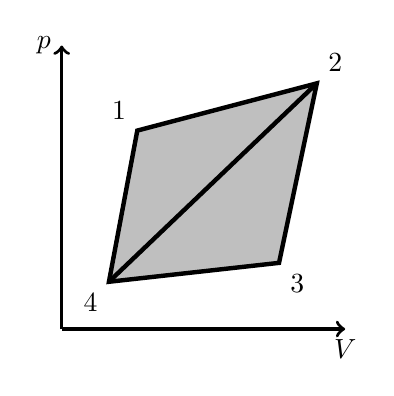
\begin{tikzpicture}[scale=1.2]
                \draw[very thick,->]
                    (0,0) -- (3,0) node[below] {$V$};
                \draw[very thick,->]
                    (0,0) -- (0,3) node[left] {$p$};
                \draw[fill=lightgray,ultra thick]
                    (0.5,0.5) node[below left] {4}
                    -- (2.3,0.7) node[below right] {3}
                    -- (2.7,2.6) node[above right] {2}
                    -- (0.8, 2.1) node[above left] {1} -- cycle;
                \draw[ultra thick]
                    (0.5,0.5) -- (2.7,2.6);
            \end{tikzpicture}
        \end{figure}
        \answer{$\eta=\eta_1+\eta_2-\eta_1\eta_2$}

    \item
        (Irodov) Um ciclo termodinâmico para um gás ideal consiste em uma
        isoterma, um processo politrópico e uma adiabata, com o processo
        isotérmico ocorrendo à temperatura máxima do ciclo. Encontre a
        eficiência $\eta$ deste ciclo sabendo que a a temperatura máxima é
        $\alpha$ vezes a temperatura mínima do ciclo.
        \answer{$\eta=1-\frac{\alpha-1}{\alpha\log\alpha}$}

    \item
        O nome de temperatura termodinâmica e a utilização da letra $T$ para a
        temperatura na equação de estado do gás ideal não é coincidência.
        Partindo das equações
        $$pV=NRT,\quad U=\frac{NRT}{\gamma-1}$$
        \begin{enumerate}
            \item
                Construa o ciclo de Carnot através de duas isotermas e duas
                adiabáticas para concluir que $T$ é uma escala de temperatura
                termodinâmica.
            \item
                Escreva uma expressão para a entropia do gás ideal em termos da
                energia interna $U$, volume $V$, número de moléculas $N$,
                coeficiente de Poisson $\gamma$ e uma constante arbitrária.
                \answer{
                    $S=\frac{NR}{\gamma-1}
                    \log\frac{UV^{\gamma-1}}{\Phi N^\gamma}$
                }
        \end{enumerate}

    \item
        Mostre que se a pressão de um sistema pode ser escrita $p=Tf(V)$ então a
        energia interna $U$ depende apenas da temperatura $T$. Conclua que a
        equação para a energia interna do gás ideal segue da equação de estado
        para a pressão e da suposição que $C_V$ é independente da temperatura.
        \answer{$\pd{U}{V}{T}=T\pd{p}{T}{V}-p$}

    \item
        O ciclo de Stirling para um gás ideal é definido 
        \begin{itemize}
            \item 
                $1\rightarrow2$ compressão isotérmica por um fator $r$
            \item
                $2\rightarrow3$ aquecimento isocórico até $T_H$
            \item
                $3\rightarrow4$ expansão isotérmica
            \item
                $4\rightarrow1$ resfriamento isocórico até $T_C$
        \end{itemize}
        \begin{enumerate}
            \item
                Desenhe o ciclo num diagrama $pV$.
                \answer{
                    \begin{tikzpicture}
                        \draw[very thick,->]
                            (0,0) -- (3,0) node[right] {$V$};
                        \draw[very thick,->]
                            (0,0) -- (0,2) node[above] {$p$};
                        
                        \draw
                            (0.8,0.1) -- (0.8,-0.1) node[below] {$V_0$};
                        \draw
                            (2.5,0.1) -- (2.5,-0.1) node[below] {$rV_0$};
                        \draw
                            (0.1,0.7) -- (-0.1,0.7) node[left] {$\alpha T_C$};
                        \draw
                            (0.1,1.7) -- (-0.1,1.7) node[left] {$\alpha T_H$};

                        \draw[ultra thick,fill=lightgray]
                            (2.5,{0.7*0.8/2.5}) node[right] {1}
                            plot[domain=2.5:0.8,samples=10]
                                (\x,{0.7*0.8/\x}) node[left] {2}
                            -- (0.8,1.7) node[left] {3}
                            plot[domain=0.8:2.5,samples=10]
                                (\x,{1.7*0.8/\x}) node[above] {4}
                            -- (2.5,{0.7*0.8/2.5});

                        \path[ultra thick,postaction={mid arrow}]
                            plot[domain=2.5:0.8,samples=10] (\x,{0.7*0.8/\x});
                        \path[ultra thick,postaction={mid arrow}]
                            (0.8,0.7) -- (0.8,1.7);
                        \path[ultra thick,postaction={mid arrow}]
                            plot[domain=0.8:2.5,samples=10] (\x,{1.7*0.8/\x});
                        \path[ultra thick,postaction={mid arrow}]
                            (2.5,{1.7*0.8/2.5}) -- (2.5,{0.7*0.8/2.5});
                    \end{tikzpicture}
                }
            \item
                Desenhe o ciclo num diagrama $TS$.
                \answer{
                    \begin{tikzpicture}
                        \draw[very thick,->]
                            (0,0) -- (3,0) node[right] {$S$};
                        \draw[very thick,->]
                            (0,0) -- (0,2) node[above] {$T$};
                        
                        \draw
                            (0.8,0.1) -- (0.8,-0.1) node[below] {$0$};
                        \draw
                            (2.3,0.1) -- (2.3,-0.1) node[below] {$NR\log r$};
                        \draw
                            (0.1,0.7) -- (-0.1,0.7) node[left] {$T_C$};
                        \draw
                            (0.1,1.7) -- (-0.1,1.7) node[left] {$T_H$};

                        \draw[ultra thick,fill=lightgray]
                            (0.8,0.7)
                            plot[domain=0.8:1.2,samples=10]
                                (\x,{0.7*(1.7/0.7)^((\x-0.8)/0.4)})
                                node[left] {3}
                            -- (2.7,1.7) node[right] {4}
                            plot[domain=2.7:2.3,samples=10]
                                (\x,{0.7*(1.7/0.7)^((\x-2.3)/0.4)})
                                node[right] {1} 
                            -- (0.8,0.7) node[left] {2};

                        \path[ultra thick,postaction={mid arrow}]
                            plot[domain=0.8:1.2,samples=10]
                                (\x,{0.7*(1.7/0.7)^((\x-0.8)/0.4)});
                        \path[ultra thick,postaction={mid arrow}]
                            (2.3,0.7) -- (0.8,0.7);
                        \path[ultra thick,postaction={mid arrow}]
                            plot[domain=2.7:2.3,samples=10]
                                (\x,{0.7*(1.7/0.7)^((\x-2.3)/0.4)});
                        \path[ultra thick,postaction={mid arrow}]
                            (1.2,1.7) -- (2.7,1.7);
                    \end{tikzpicture}
                }
            \item
                Encontre a eficiência $\eta$ do ciclo supondo que ele ocorre num
                gás ideal de coeficiente de Poisson $\gamma$ e mostre que é
                menor do que a eficiência de Carnot operando entre $T_C$ e
                $T_H$.
                \answer{
                    $\eta=1-\frac{T_C+\Delta T}{T_H+\Delta T},
                    \quad\Delta T=\frac{T_H-T_C}{(\gamma-1)\log r}$
                }
        \end{enumerate}
        Para os gráficos introduza constantes para que marcações nos eixos façam
        sentido.

    \item
        (SOIF 2022) Um físico passará o inverno isolado dentro de casa e
        projetará um sistema de aquecimento para garantir o seu conforto. O
        sistema visa manter a temperatura no interior da casa em $T_C=278
        \,\mathrm K$, enquanto a temperatura do ambiente externo é $T_F=263
        \,\mathrm K$. O sistema dispõe de uma lareira que pode servir de
        reservatório térmico de temperatura $T_Q=600\,\mathrm K$. Temos o
        objetivo de transferir uma quantidade de calor $Q$ para dentro da casa
        com o menor custo energético possível. Assumindo que podemos transferir
        calor da lareira tanto do interior quanto para o exterior da casa, qual
        a menor quantidade de calor $Q'$ que precisa ser extraida da lareira
        para que isso seja possível?
        \answer{$Q'=\frac{T_Q(T_C-T_F)}{T_C(T_Q-T_F)}Q=0{,}096Q$}

    \item
        Considere dois objetos de capacidade térmica $C_1$ e $C_2$ com
        respectivas temperaturas $T_1$ e $T_2$. Utilizando apenas um conjunto de
        máquinas térmicas sem fontes de calor externas, qual a menor temperatura
        de equilíbrio possível para estes objetos? Comente sobre o caso $C_2\ll
        C_1$.
        \answer{
            $T_0=\left(T_1^{C_1}T_2^{C_2}\right)^\frac{1}{C_1+C_2}
            \approx T_1+\frac{C_2}{C_1}T_1\log\frac{T_2}{T_1}$
        }

    \item
        Considere um cilíndro adiabático vertical de área de seção transfersal
        $A$. No interior deste há uma certa quantidade de fluido. Coloque um
        pistão adiabático de massa $m$ e área também $A$ que se move sem atrito
        pelo cilíndro. Dado que a gravidade local é $g$ e a pressão atmosférica
        é $p_0$, encontre a pressão do gás no equilíbrio termodinâmico.
        \answer{$p=p_0+\frac{mg}{A}$}
\end{enumerate}
